\documentclass{beamer}

\setlength{\parskip}{\baselineskip}
\setlength{\parindent}{0pt}
\usepackage{default}
\usepackage{tabularx}
\usepackage{hyperref}
\usepackage{graphicx}

\title{\huge{COSSE and beyond}}
\author{Manuel Baumann, Slobodan Milovanovi\'{c}}
\titlegraphic{
   
\includegraphics[scale=0.08]{images/TU_Delft_logo1.png}\hspace{3cm}
\includegraphics[scale=0.1]{images/UppU_logo.png}}
\date{\footnotesize{February 11, 2014}}
\begin{document}

\frame{\titlepage}
\begin{frame}
\frametitle{Outline}
\tableofcontents
\end{frame}


\section{The COSSE almuni program}
\begin{frame}
\frametitle{Erasmus Mundus Students and Alumni Association (EMA)}
\begin{itemize}
 \item \href{http://www.em-a.eu/}{http://www.em-a.eu/} 
\end{itemize}

\end{frame}

\section{COSSE best practice guide}
\begin{frame}
\frametitle{A COSSE best practice guide}
 bla
\end{frame}

\section{COSSE - What's next?}
\subsection{Boba's PhD}
\begin{frame}
\frametitle{COSSE - What's next?}
 TODO: Boba's PhD project (10mins)
\end{frame}
\subsection{Manuel's PhD}
\begin{frame}
\frametitle{Fast iterative solution of the time-harmonic elastic wave equation at multiple frequencies}
\begin{columns}
\begin{column}{0.6\textwidth}
 The project setting:
 \begin{itemize}
  \item 4 years
  \item supervisors: Kees Vuik, Martin van Gijzen
  \item founded by \textsc{Shell}
  \item doctoral education through TU Delft graduate school
  \item practical application in the field of geoscience
 \end{itemize}
\end{column}
\begin{column}{0.4\textwidth}
\begin{figure}[t]
\centering
\vspace{-1.3cm}
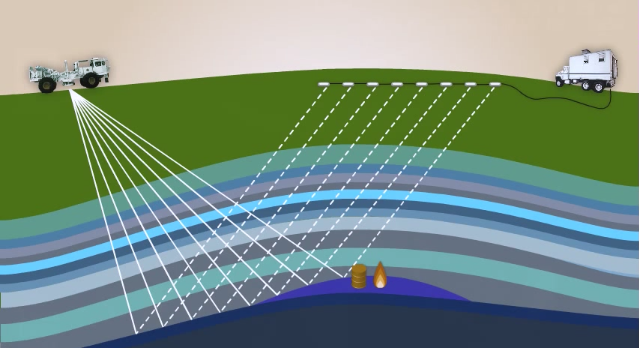
\includegraphics[width=\textwidth]{images/snapshot1.png}
\end{figure}
\end{column}
\end{columns}

\end{frame}
\begin{frame}
\frametitle{Fast iterative solution of the time-harmonic elastic wave equation at multiple frequencies}
\framesubtitle{The underlying mathematics}
Wave propagation in elastic materials:
\begin{align*}
 -\color{blue}\omega_k^2\color{black} \rho(\mathbf{x}) \mathbf{u} - \nabla \cdot \sigma(\mathbf{u}) = \mathbf{s}, \quad \mathbf{x} \in \Omega \subset \mathbb{R}^{2,3},
\end{align*}
where
\begin{itemize}
 \item unknown displacement vector $\mathbf{u}(\mathbf{x})$
 \pause
 \item many frequencies $\color{blue}\omega_k\color{black}, k=1,...,n_\omega$
 \pause
 \item material density $\rho(\mathbf{x})$
 \pause
 \item stress tensor
 \begin{align*}
   \sigma(\mathbf{u}) \equiv \lambda(\mathbf{x}) \left( \nabla \cdot \mathbf{u} \right) + 2 \mu(\mathbf{x}) \epsilon(\mathbf{u}), \quad  \epsilon(\mathbf{u}) \equiv \frac{1}{2} \left( \nabla \mathbf{u} + \left( \nabla \mathbf{u}\right)^T \right)
 \end{align*}
\end{itemize}

\end{frame}

\begin{frame}
\frametitle{Fast iterative solution of the time-harmonic elastic wave equation at multiple frequencies}
\framesubtitle{The underlying mathematics}
FEM discretization (including BC) yields
\begin{align*}
(K + i \color{blue}\omega_k\color{black} C - \color{blue}\omega_k^2\color{black} M)\underline{\mathbf{u}} = \underline{\mathbf{s}},
\end{align*}
which can be re-arranged as,
\begin{align*}
\left[\begin{pmatrix} i M^{-1}C & M^{-1}K \\ I & 0\end{pmatrix} - \color{blue}\omega_k\color{black} \begin{pmatrix} I & 0 \\ 0 & I\end{pmatrix} \right] \begin{pmatrix} \color{blue}\omega_k\color{black} \underline{\mathbf{u}} \\  \underline{\mathbf{u}}\end{pmatrix} = \begin{pmatrix} M^{-1}\underline{\mathbf{s}} \\ 0\end{pmatrix}.
\end{align*}
\end{frame}

\begin{frame}
\frametitle{Fast iterative solution of the time-harmonic elastic wave equation at multiple frequencies}
\framesubtitle{The underlying mathematics}
The last equation can be written as a \color{blue}shifted linear system\color{black},
\begin{align*}
 (A - \color{blue}\omega_k\color{black} I)\mathbf{x}_k = \mathbf{b}, \quad k = 1,...,n_\omega,
\end{align*}
where $ \omega_k \in \mathbb{C}$.

Krylov subspace methods are \textbf{the} solution algorithm, since:
\begin{align*}
\mathcal{K}_m(A,\mathbf{b}) \equiv \text{span}\{\mathbf{b}, A\mathbf{b},...,A^{m-1}\mathbf{b}\} = \mathcal{K}_m(A-\omega_k I,\mathbf{b}) 
\end{align*}
\end{frame}
\begin{frame}
\frametitle{Fast iterative solution of the time-harmonic elastic wave equation at multiple frequencies}
\framesubtitle{The underlying mathematics}
In \texttt{GMRES}, it holds
\begin{align*}
A V_m &= V_{m+1} \underbar{H}_m
\end{align*}
and, therefore, for the shifted systems,
\begin{align*}
(A - \omega_k I) V_m &= V_{m+1} (\color{blue}\underbar{H}_m - \omega_k \underbar{I}_m\color{black}).
\end{align*}
\pause
\begin{itemize}
 \item Compute $V_m$ via Arnoldi algorithm \textbf{once},
 \item Use \color{blue}shifted Hessenberg matrix \color{black} to approximate solution of shifted systems
\end{itemize}

\end{frame}
\begin{frame}
\frametitle{Fast iterative solution of the time-harmonic elastic wave equation at multiple frequencies}
\framesubtitle{The underlying mathematics}
\begin{columns}
\begin{column}{0.6\textwidth}
Challenges:

 \begin{itemize}
  \item short-reccurence (IDR)
  \item preconditioning (flexible Krylov)
  \item memory-efficient (HPC)
 \end{itemize}
\end{column}
\begin{column}{0.4\textwidth}
\begin{figure}[t]
\centering
%\setbeamercovered{transparent}
\includegraphics<1>[scale=0.3]{images/dens_middleEast}
\includegraphics<2>[scale=0.25]{images/middleEast5.png}
\end{figure}
\end{column}
\end{columns}
\end{frame}
\subsection{Some others}
\begin{frame}
\frametitle{What our fellow students do now}
Let's finish with some more examples (unsorted, unbiased)...
\vspace{-0.3cm}
\begin{description}[manymanymanypeople]
 \pause
 \item[Miguel Romero] Chemical and process engineering at BASF, Heidelberg
 \pause
  \item[Xiao Liang] PhD student, \href{http://www.molgen.mpg.de/IMPRS}{Max Planck Institute for Computational Biology}, Berlin
 \pause
 \item[Martin Ambrozic] Works now at \href{http://www.abelium.eu/raziskave}{'abelium'} in Ljubljana
 \pause
 \item[Firat Haciahmetoglu] \href{http://onderwijsaanbod.kuleuven.be/opleidingen/e/SC\_50841972.htm\#bl=01,02,03,04,05\&activetab=opbouw}{Bachelor of Philosophy}, KU Leuven, Belgium 
  \pause
  \item[\href{http://www.kth.se/en/studies/master/em/cosse/programme/degree-projects-1.388741}{Carolyn Langen}] PhD student in \href{http://www.bigr.nl/website/index.php?page=content&subpage=about}{Biomedical Imaging Group, Erasmus MC Rotterdam}
 \pause
  \item[Anna Babaryka] IT-consultant at \href{http://idealapps.se/}{idealapps}, Stockholm
  \pause
  \item[Elmarie van Heerden] PhD in South Africa \& Oxford U on \href{http://www.skatelescope.org/}{SKA radio telescope}
  \pause
  \item[Matthew The] Open source developer at \href{http://www.scilifelab.se/about-us/}{SciLifeLab}, Stockholm
  \pause
  \item[Shiyang Hu] PhD at FAU on Dark-Field Imaging 

\end{description}
\end{frame}

\end{document}
